
\documentclass[
				oneside,
				11pt, a4paper,
				footinclude=true,
				headinclude=true,
				cleardoublepage=empty
]{scrbook}

\usepackage[utf8]{inputenc}
\usepackage{lipsum}
\usepackage[linedheaders,parts,pdfspacing]{classicthesis}
\usepackage{amsmath}
\usepackage{amsthm}
\usepackage{acronym}
\usepackage{algorithm}
\usepackage{algpseudocode}
\usepackage{tikz}
\usetikzlibrary{shapes}
\usetikzlibrary{positioning,arrows}
\usetikzlibrary{decorations.pathreplacing} 

\newtheorem{theorem}{Theorem}
\newtheorem{proposition}[theorem]{Proposition}


\author{João Valença}
\title{Visualisation and Analysis of Geographic Information: Algorithms and Data Structures}

\textwidth = 370 pt


\begin{document}
\maketitle	

\setcounter{tocdepth}{2} % <-- 2 includes up to subsections in the ToC
\setcounter{secnumdepth}{3} % <-- 3 numbers up to subsubsections
\tableofcontents 

\setcounter{page}{0}
\pagenumbering{roman}
\vspace*{0.1cm}
\section*{\huge Abstract}

In recent years, Geographic Information Systems have witnessed a large increase in data availability. There is a need to process a large amount of data before it can be managed and analysed. This project aims to develop an application operating through a Web platform in order to allow for a low cost and simplified integration, management and manipulation of georeferenced information. Special emphasis is given to the implementation of efficient clustering algorithms for finding a representative set of points in a map. In the thesis, this representation problem is formulated as two classic optimisation problems: the \emph{$k$-center} and the \emph{geometric disk cover}. The approaches covered in this thesis include exact algorithms for solving the \emph{k-centre} problem, as well as approximation algorithms and heuristic methods to solve the \emph{geometric disk cover} problem. The algorithms are experimentally evaluated in a wide range of scenarios.

\subsection*{\large Keywords}

Geographic Clustering, Computational Geometry Algorithms, Coverage Problems, Real-Time Applications.

\vspace*{0.6cm}

\section*{\huge Resumo}

Nos últimos anos, os Sistemas de Informação Geográfica têm assistido a um grande aumento na quantidade de dados disponíveis. De facto, existe uma necessidade de encontrar uma maneira eficiente de processar grandes quantidades de dados para que tanta informação possa ser facilmente gerida e analisada. Este projeto visa desenvolver uma aplicação para uma plataforma Web, de modo a obter uma integração simples e de baixo custo que manipule e analise dados georeferenciados. Uma ênfase especial é dada à implementação de algoritmos para encontrar um conjunto representativo de pontos num mapa. Nesta tese, o problema de representação é formulado como dois problemas de optimisação clássicos: \emph{$k$-centre} e \emph{geometric disk cover}. As abordagens descritas nesta tese incluem algoritmos exactos para resolver o problema do \emph{k-centre}, bem como algoritmos de aproximação e métodos heurísticos para resolver o problema de \emph{geometric disk cover}. Os algoritmos são experimentalmente avaliados numa grande seleção de cenários.

\subsection*{Palavras-chave}

Clustering Geográfico, Algoritmos de Geometria Computacional, Problemas de Cobertura, Aplicações em Tempo Real.

\vfill
\chapter{Introduction}
\label{chap:intro}
\lhead{Chapter \ref{chap:intro}. \emph{Introduction}} % This is for the header
\paragraph{}
In recent years, there has been a large increase in both the quantity and availability of geographic data. This new availability of such large quantities of data has prompted a similar rise on the number of applications to capture, store, manipulate and analyse this data.
A lot of these applications share the need to visualise the geographic information in such a way that it can be easily understood by a human.
This is usually done by displaying points of interest on a map so that their relative position or direction can be easily interpreted without much thought by the user.
\\
One obstacle when representing large amounts of geographic data is that the sheer volume of points to display can be overwhelming for a human, as well as computationally intensive to render for a machine. As such, there is a need to develop and implement a viable way to reliably calculate and display a subset of geographic points, whilst keeping a degree of representability of the larger set, so that as little information as possible is absent when the representative subset is shown.
\\
The purpose of this project is to research and develop a real-time algorithm that can analyse geographic data provided by a geographic information system (GIS) infrastructure developed and maintained at Smartgeo. More precisely, the developed algorithm will have to be able to aggregate and select geographic points according to a given a set of criteria.
\\
\begin{figure}[H]
	\centering
	\begin{minipage}{0.4\linewidth}
		\centering
		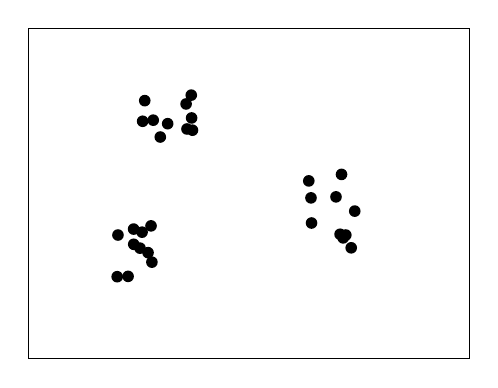
\begin{tikzpicture}[scale=1.4]
			\draw (-0.5,-0.4) rectangle (3.5,2.6);
			
			\fill (0.456,0.778)circle (1.5pt);
			\fill (0.622,0.478)circle (1.5pt);
			\fill (0.457,0.64)circle (1.5pt);
			\fill (0.614,0.807)circle (1.5pt);
			\fill (0.314,0.724)circle (1.5pt);
			\fill (0.533,0.75)circle (1.5pt);
			\fill (0.514,0.605)circle (1.5pt);
			\fill (0.307,0.346)circle (1.5pt);
			\fill (0.406,0.349)circle (1.5pt);
			\fill (0.587,0.564)circle (1.5pt);
			
			\fill (2.065,1.061)circle (1.5pt);
			\fill (2.045,1.215)circle (1.5pt);
			\fill (2.292,1.07)circle (1.5pt);
			\fill (2.381,0.724)circle (1.5pt);
			\fill (2.43,0.608)circle (1.5pt);
			\fill (2.342,1.274)circle (1.5pt);
			\fill (2.329,0.731)circle (1.5pt);
			\fill (2.462,0.941)circle (1.5pt);
			\fill (2.357,0.698)circle (1.5pt);
			\fill (2.07,0.833)circle (1.5pt);
			
			\fill (0.765,1.734)circle (1.5pt);
			\fill (0.557,1.943)circle (1.5pt);
			\fill (0.698,1.613)circle (1.5pt);
			\fill (0.634,1.766)circle (1.5pt);
			\fill (0.979,1.993)circle (1.5pt);
			\fill (0.99 ,1.675)circle (1.5pt);
			\fill (0.538,1.756)circle (1.5pt);
			\fill (0.932,1.913)circle (1.5pt);
			\fill (0.982,1.786)circle (1.5pt);
			\fill (0.94 ,1.686)circle (1.5pt);
		\end{tikzpicture}
		\caption*{\footnotesize Original Set}
		\label{fig:badrep}
	\end{minipage}
	\hspace{1cm}
	\begin{minipage}{0.4\linewidth}
		\centering
		\begin{tikzpicture}[scale=1.4]
		\draw (-0.5,-0.4) rectangle (3.5,2.6);
		
		\fill (0.765,1.734)circle (1.5pt);
		\fill (0.514,0.605)circle (1.5pt);
		\fill (2.292,1.07)circle (1.5pt);
		\end{tikzpicture}		
		\caption*{\footnotesize Representative Subset}
		\label{fig:goodrep}
	\end{minipage}
	\caption{Example of a Representative Set}
	\label{fig:rep}
\end{figure}
\paragraph{}
This thesis aims to research, develop, and analyse different algorithms to choose a representative subset of geographic points, whilst being able to dynamically change that set of points via zooming or panning over a geographic region containing a large amount of geographical data. Should optimal solution algorithms prove too slow, heuristic approaches will be employed. Heuristic algorithms will have their solution quality and speed benchmarked against implicit enumeration algorithms.
Whichever algorithm is deemed the best will be implemented in the web framework via the \emph{WFS} and \emph{WMS} web mapping standards.
\paragraph{}
This report is organized as follows:
Chapter \ref{chap:theory} - \nameref{chap:theory} defines the base theoretical concepts, such as a notion of representativeness, as well as some useful structures used in the algorithms. Chapter \ref{chap:sota} - \nameref{chap:sota} analyses previous related work. Chapter \ref{chap:algos} - \nameref{chap:algos} describes the implicit enumeration algorithms implemented so far, as well as an analysis on their time and space complexities. Chapter \ref{chap:future} - \nameref{chap:future} describes the direction of the heurisitc algorithms to be developed in the second half of the thesis. 
\input{cstudy}
\cleardoublepage
\chapter{Exact Algorithms for the k-Centre Problem}
\label{chap:algos}
%\lhead{Chapter \ref{chap:algos}. \emph{\nameref{chap:algos}}} % This is for the header

\begin{change}
This chapter describes two possible algorithms that solve the k-centre problem. The goal of this problem is to, given a set of points $N$, find the subset of centroids of cardinality $k$ that minimises the distance between the farthest point in $N$ and its closest centroid. 

Both algorithms use an incremental branch-and-bound approach for implicit enumeration of the centroid subsets. The first algorithm is a naïve implementation of a branch-and-bound algorithm and uses simple loops over arrays for point location queries. The second algorithm builds and uses Delaunay triangulations to achieve more efficient point location queries. At the end of this chapter, these algorithms, as well as an implementation of the Integer Linear Programming formulation described in Section \ref{alg:ilp}, are experimentally tested in a set of benchmark instances.

\end{change}
\section{Naïve Branch-and-Bound}
\label{alg:bb}

\begin{change}
A more sophisticated approach to the problem is to use a branch-and-bound method.
In our approach, the assignment of non-centroids to their correct centroids is built incrementally.

\citet{incrementalcov} solve the \emph{k-centre} problem heuristically using local search. Their method describes algorithms to incrementally insert and remove centroids from a set of points, and update the centroid assignment only in the geometrical area surrounding the changed point. This method allows for small modifications on an already valid solution, and the techniques for updating the objective function upon insertion and removal of points can be used in an incremental branch-and-bound method to speed up the computation between branches, without having to calculate the full point assignment for every iteration of the algorithm, whilst still implicitly enumerating all possible combinations. 

To solve the problem incrementally, at each step of the recursive tree, one of the available points is considered. A decision is then taken of whether the point is a centroid or a non-centroid. According to which decision is taken, the objective function and the centroid assignment is updated accordingly. This is done until all the centroids have been chosen and a solution is found at the end of the branch. The best solution in all the branches is the optimal value for the k-centre problem.
\end{change}

\subsection{Branching}
As stated above, branching the tree involves updating the assignment between new points and/or new centroids, as well as updating the objective function. The following procedures explain in detail how to do so.
\paragraph{Inserting a Centroid}
To insert a centroid $c$, the established non-centroids which are closer to $c$ than their current centroid must be checked, and change their assignment to $c$.
Since non-centroids only change assignment to centroids closer to them, inserting a centroid means that the objective function either decreases in value or stays the same.\\
After inserting a centroid, if the farthest non-centroid is reassigned, all non-centroids must be checked to see which one now maximises the objective function.
This step compares all non-centroids to the new centroid $c$, taking $\Theta(N)$ time.

\paragraph{Inserting a Non-Centroid}
Inserting a non-centroid $n$ only requires finding which of the current centroids is the closest to $n$. Updating the objective function is a matter of testing whether the distance between $n$ and its centroid is larger than the current maximum.
Inserting a non-centroid cannot produce a better objective function, since it will either decrease or maintain the current value. 
This step compares the distance between point $n$ and all centroids, taking $\Theta(k)$ time.
\paragraph{}
After a branch is fully calculated, it is necessary to backtrack to the parent state, either by removing a centroid, or a non-centroid.
\paragraph{Removing a Centroid}
Removing a centroid $c$ means redistributing the values assigned to $c$ to their respective closest centroids in the remaining set. \\
The value function either increases or maintains, since the distance for all points previously assigned to $c$ will increase, potentially above the current value for the objective function.
Removing a centroid $c$ means comparing all non-centroids assigned to $c$ to all the other centroids. This step takes $\Theta(NK)$ time to execute. Alternatively, if the assignment state is saved before inserting the centroid, recovering it requires only retrieving the state, which means, in the worst and best cases copying an array of size $N$, which takes $\Theta(N)$ time at the expense of additional $\Theta(N)$ memory space.

\paragraph{Removing a Non-Centroid}
In order to remove a non-centroid $n$, we only need to update the objective function. If point $n$ maximises the objective function, the second farthest point from its centroid, the new maximiser, must be found.
Removing a non-centroid can either decrease or maintain the value of the objective function.
Removing a non-centroid $n$ means that the next farthest point from its centroid must be found. This can be done by checking all distances between the non-centroids and their respective centroids, taking $\Theta(N)$ time. Alternatively, one can save the previous value for the objective function, as well as the maximiser. Retrieving the previous value can be done in $\mathcal{O}(1)$ time at the expense of additional $\Theta(1)$ memory space.
\subsection{Bounds}
\label{sec:bounds}
At all steps in the branching, the lower bound for the value of the objective function in the current branches is calculated. If the lower bound is larger than an already calculated upper bound, then there is no purpose in further exploring the current branch. In a minimisation problem, the upper bound can be the best solution found until that point in time.

\paragraph{Lower Bound}
After each insertion, centroid or non-centroid, one can assume that, the best case scenario, all the points not yet inserted will be centroids. This would hypothetically decrease the value the most. If this value is larger than the best value found, then there is no possible assignment that will improve the current solution in the current branch, and the branch can be pruned.
\section{Delaunay Assisted Branch-and-Bound}
\label{alg:da}

Most of the operations in the branch-and-bound approach described in Section \ref{alg:bb} have at least linear time complexity for both the best and expected cases. We can speed these up by implementing incrementally built Delaunay triangulations, which can be used to accelerate point location queries. To aid the calculations, the points are pre-processed and sorted by a Hilbert Curve approximation of a sufficiently high order.

\paragraph{Inserting a Centroid}
In order to take advantage of Delaunay triangulations, each time a centroid is chosen, it must be included in the Delaunay triangulation. This means that the triangulation must be updated. Inserting a point in a triangulation with $K$ vertices using the Bowyer-Watson algorithm described in Section \ref{sect:dtconst} takes an estimated $\mathcal{O}(\log{K})$ for a uniformly distributed set of points \cite{tricomplex}.
After a centroid $c$ is included in a Delaunay triangulation, it is possible to know which other centroids are its Voronoi neighbours. This is due to the duality between Delaunay triangulations and Voronoi diagrams.
Since Voronoi diagrams partition the space into regions by distance to the centroids, we only need to check the subset of non-centroids assigned to the direct neighbours of $c$ to find which points should change assignment to $c$. 
This property lowers the expected number of comparisons to make. Since the average number of Voronoi neighbours per centroid in any given diagram cannot exceed six \cite{tricard2,tricard1}, the number of points to be compared in a uniformly distributed set of non-centroids should not include all non-centroids, but only a small fraction of them.
Despite the lower number of comparisons, the worst-case time complexity still takes $\mathcal{O}(N)$ time to complete, and in the worst case scenario it can still require a check through all non-centroids, which can all be neighbours of $c$.
If the objective function maximiser is assigned to $c$, all non-centroids can be candidates to become the new maximiser, so a linear search through all the non-centroids must be done, to see which one is now the farthest away from its centroid.

\paragraph{Inserting a Non-Centroid}
Since there is a triangulation built, using the centroids as its vertices, finding the closest centroid $c$ to a new non-centroid $n$ is simply a matter of using the greedy routing algorithm to find $c$ \cite{greedyroute}.
The greedy routing algorithm has a worst-case time complexity of $\mathcal{O}(K)$. This happens when the search starts from the farthest centroid from $n$, and all centroids are either in the direction of $n$, or are neighbours of the centroids that are. 
The last centroid returned by the greedy routing algorithm can be used to start the new query. Since the points are inserted ordered by a Hilbert curve approximation, each consecutive point should minimise the position variation from the last.
This means that, ideally, each inserted non-centroid $n$ will be close to its respective optimally positioned centroid $c$, and it will only need to calculate the distances to the neighbours of $c$ in order to guarantee that $c$ is indeed the correct centroid.
The aforementioned property of the average six neighbours for each centroid means that the expected time for a query starting at the right centroid would be $\mathcal{O}(1)$. This represents the best case scenario, and is heuristically approximated by the Hilbert curves. The time complexity of inserting one non-centroid is still $\mathcal{O}(K)$ for the worst case. 
However, the insertion of a large number of uniformly distributed points \emph{should} behave closer to $\mathcal{O}(\sqrt{K})$ time per point. If a rectangular area has $N$ points, the longest path would be a diagonal. The diagonal, like the sides, will have close to $\sqrt{N}$ number of points, in an area with a sufficiently good uniformity of points in it.

\paragraph{Removing a Centroid}
Removing a centroid $c$ means removing it from the Delaunay triangulation and redistributing all points assigned to $c$ across its neighbours.
Since all points are inserted in the triangulation in a LIFO order, removing a point from a triangulation is a matter of retrieving the previous state. We can do this by storing all new edges and triangles in a stack upon construction, and retrieve them upon removal, without the need of recalculating anything. Since inserting a centroid $c$ takes expected $\mathcal{O}(\log{K})$ time \cite{tricomplex}, and removing it will take exactly the same higher level operations (in reverse order), it can also be done in expected $\mathcal{O}(\log{K})$ time, without the need to do extra calculations.
Likewise, redistributing the points assigned to $c$ takes retrieving the previous state. Each change in assignment can be saved in a stack upon insertion, and retrieving it can be done by popping the stack.
This step also takes $\mathcal{O}(N)$ time, since all points can change assignment. However, using a stack limits the number of operations to only those that changed upon insertion, which in an uniform distribution, means an expected time complexity of $\mathcal{O}(N/K)$.

\paragraph{Removing a Non-Centroid}
Removing a non-centroid $n$ only requires recovering the second farthest point if $n$ is currently the farthest point, otherwise, no operations besides erasing $n$'s assignment, taking $\mathcal{O}(1)$ time and memory.
\paragraph{Bounds}
The same lower bound described in Section \ref{sec:bounds} can be applied in this approach. Both algorithms have the same time complexity of $\mathcal{O}(N)$ for computing the bound.

These steps occur at each iteration of the branch-and-bound algorithm, and each is performed potentially $2^N$ times for both approaches.
Despite having the same worst-case time complexity as the branch-and-bound algorithm described in Section \ref{alg:bb}, the expected time complexity for the Delaunay assisted approach is smaller. This approach should have better performance when a large number of centroids are needed.
This is especially true since maintaining a valid Delaunay triangulation through all the centroid permutations, as well as the Hilbert sorting, takes a computing cost. This extra overhead will have a negative impact in the performance in the smaller instances of the problem.
\section{Algorithm Comparison}

\subsection{Time Complexity}

Each of the procedures mentioned in the previous Section are performed at each step of the recursive tree. At each step the bound is also calculated, which takes $\mathcal{O}(N)$ time. Table \ref{tab:exptime} shows the time complexities for each procedure in both algorithms. The values presented at the row corresponding to the average case of the Delaunay-assisted algorithm are conjectured and need to be shown in a more formal manner.
\begin{table}[H]
\begin{center}
\begin{tabular}{|c|c|c|c|c|}
	\hline
	\multirow{2}{*}{Algorithm}	& \multicolumn{2}{c|}{Insert}	& \multicolumn{2}{c|}{Remove}	\\ \cline{2-5}
								& Centroid		& Non-Centroid	& Centroid		& Non-Centroid	\\ \hline
				Naïve BB		& $\Theta(N)$ & $\Theta(K)$ 	& $\Theta(N)$ & $\mathcal{O}(1)$ \\ \hline\hline
				Del. Assisted BB	
				& \multirow{2}{*}{$\mathcal{O}(\log{K}+N/K)$}
				& \multirow{2}{*}{$\mathcal{O}(\sqrt{K})$}
				& \multirow{2}{*}{$\mathcal{O}(N/K)$ }
				& \multirow{2}{*}{$\mathcal{O}(1)$}\\
				Average Case & & & & \\ \hline
		Del. Assisted BB 
				& \multirow{2}{*}{$\mathcal{O}(K+N)$}
				& \multirow{2}{*}{$\mathcal{O}(K)$}	
				& \multirow{2}{*}{$\mathcal{O}(N)$} 
				& \multirow{2}{*}{$\mathcal{O}(1)$}\\ 
				Worst Case 	& & & & \\ \hline
\end{tabular}
	\captionof{table}{Time complexities for the various operations in a uniformly distributed point set}
	\label{tab:exptime}
\end{center}
\end{table}
\subsection{Experimental Results}
\paragraph{}
In this section, we analyse empirically the time spent calculating the solutions to different sizes of the problem. 
\subsubsection*{Methodology and Set-up}
The test cases are sets of uniformly distributed points generated with a fixed seed. Each test was repeated 10 times with different sets of points. The same sets and machine were used to test the three algorithms.

Both branch-and-bound approaches were implemented using \emph{C++} and compiled using \emph{g++ 4.9.2}. The integer linear programming version had the data preprocessed using \emph{python 2.7.9} and was solved using the \emph{GLPK LP/MIP v4.55} solver. The programs were ran on a machine with a Intel i7 Dual-Core, 2GHz processor, with a 8 GB, 1600 MHz memory and Arch Linux 3.14.4 x64 as its operating system.

\subsubsection*{Effect of $N$}

The first test conducted analysed the variance in performance relative to changes in the value of $N$. It was done by changing $N$, with $K$ taking fixed fractional values of $N$. Figure \ref{fig:fixed_k} shows the results of these tests. The measures were taken in seconds and account for the pre-processing steps and the solving time, but not the input reading or output writing times. The tests were stopped at the half-hour mark. 
\begin{figure}[t] 
	\begin{subfigure}[b]{0.4\linewidth}
		\centering
		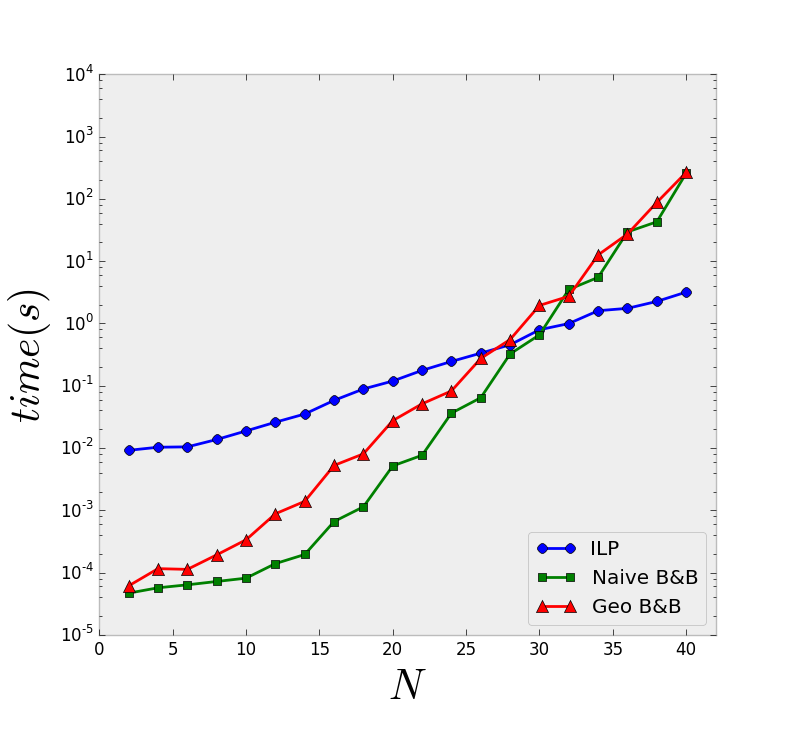
\includegraphics[width=0.9\linewidth]{Pictures/k1} 
		\caption{$K=0.25N$} 
		\label{fig:fixed_k:a} 
	\end{subfigure}%% 
	\begin{subfigure}[b]{0.4\linewidth}
		\centering
		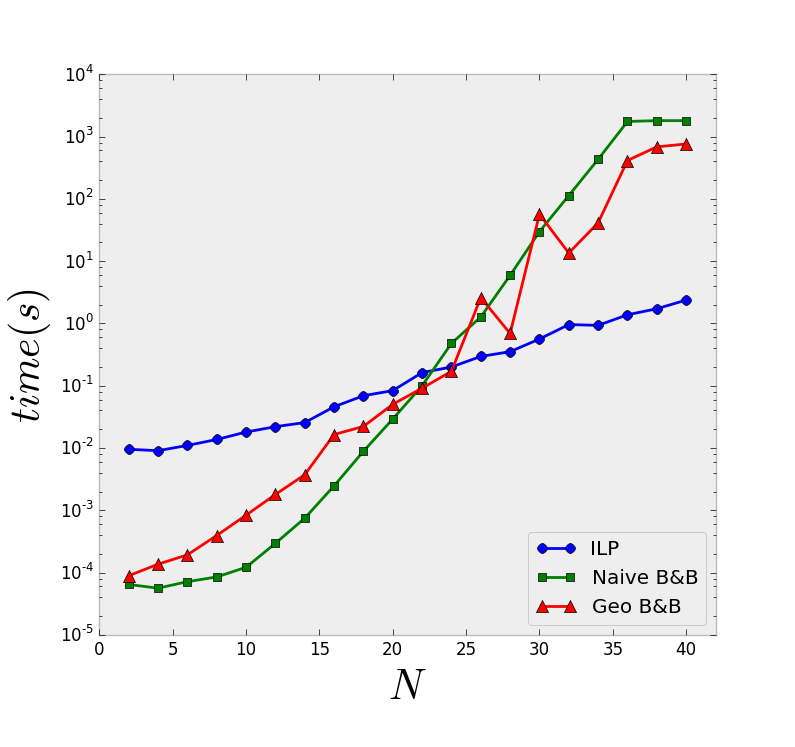
\includegraphics[width=0.9\linewidth]{Pictures/k2} 
		\caption{$K=0.5N$} 
		\label{fig:fixed_k:b} 
	\end{subfigure} 
	\begin{center}
	\begin{subfigure}[b]{0.4\linewidth}
		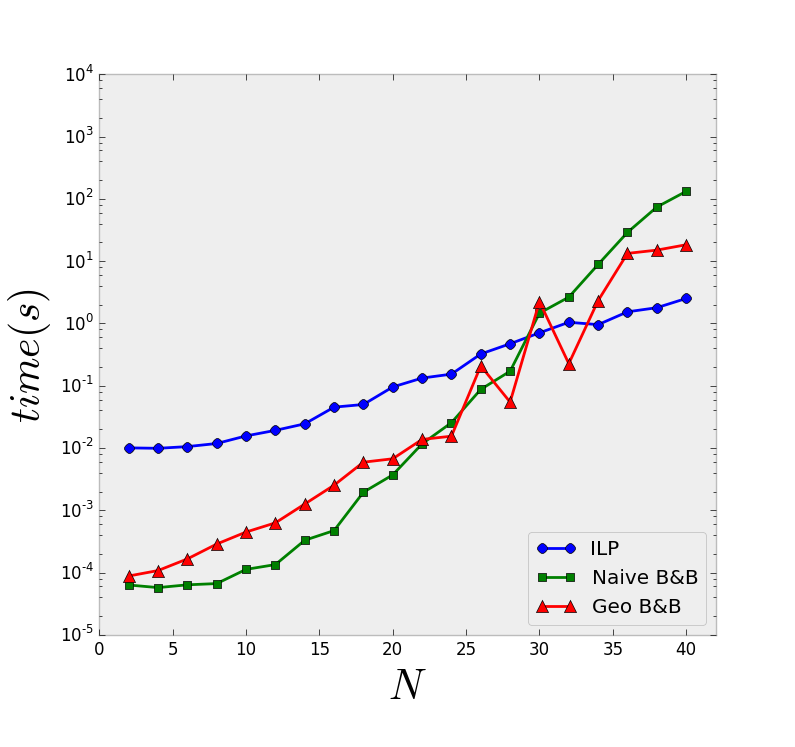
\includegraphics[width=0.9\linewidth]{Pictures/k3} 
		\caption{$K=0.75N$} 
		\label{fig:fixed_k:c} 
	\end{subfigure}
	\end{center}
	\begin{center}
    \textcolor{blue}{\cmark}\ -- Integer Linear Programming\quad   \textcolor{red}{\tmark}\ -- Delaunay Assisted B\&B\quad \textcolor{green}{\smark}\ -- Naive B\&B
    \end{center}
	\caption{CPU-time for different values of $K$ with varying values of $N$}
	\label{fig:fixed_k} 
\end{figure}


\noindent
As it can be seen, the problem solving time increases exponentially with the value of $N$, as expected.
The Integer Linear Programming Approach performs faster for larger values of $N$. Comparing the branch-and-bound approaches, these tests show that the Delaunay-assisted algorithm steadily approaches and surpasses the naïve branch-and-bound algorithm as the instance size grows.
\subsubsection*{Effect of $K$}
In this experiment, we analysed the performance of the three algorithms in dependence of parameter $K$. We fixed $N$ and varied $K$ from 2 to $N$ by steps of 2. Figure \cite{fig:fixed_n} show the results for the $N=\{10,20,30,40\}$, respectively. The tests were stopped at the half-hour mark. Figure \ref{fig:fixed_n} shows the results of these tests.
\begin{figure}[t] 
  \begin{subfigure}[b]{0.5\linewidth}
    \centering
    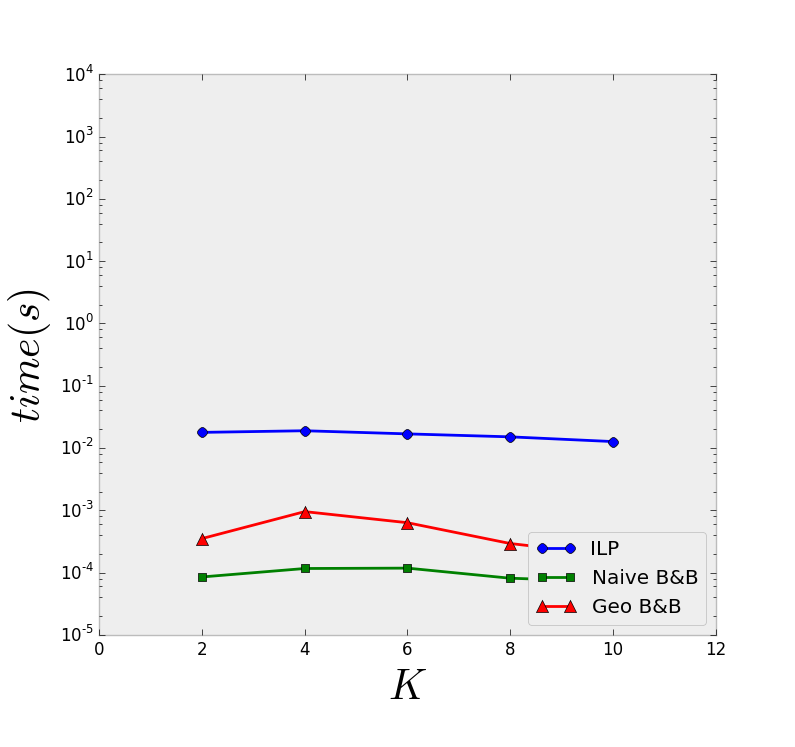
\includegraphics[width=0.9\linewidth]{Pictures/n10} 
    \caption{$N=10$} 
    \label{fig:fixed_n:a} 
    \vspace{4ex}
  \end{subfigure}%% 
  \begin{subfigure}[b]{0.5\linewidth}
    \centering
    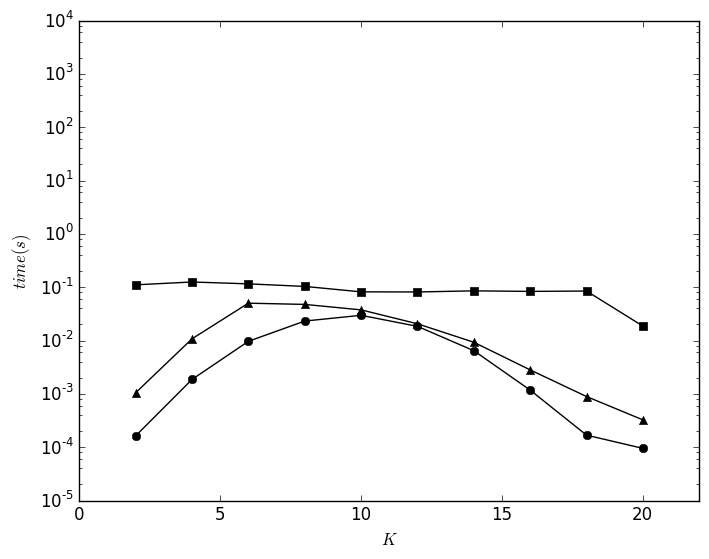
\includegraphics[width=0.9\linewidth]{Pictures/n20} 
    \caption{$N=20$} 
    \label{fig:fixed_n:b} 
    \vspace{4ex}
  \end{subfigure} 
  \begin{subfigure}[b]{0.5\linewidth}
    \centering
    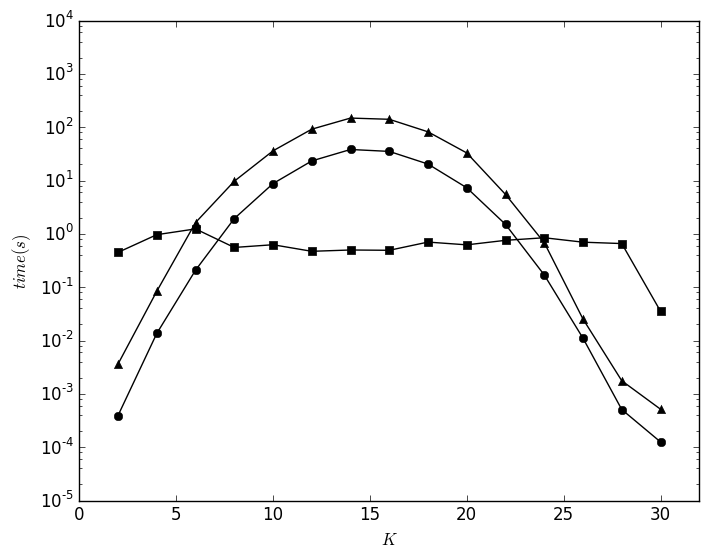
\includegraphics[width=0.9\linewidth]{Pictures/n30} 
    \caption{$N=30$} 
    \label{fig:fixed_n:c} 
  \end{subfigure}%%
  \begin{subfigure}[b]{0.5\linewidth}
    \centering
    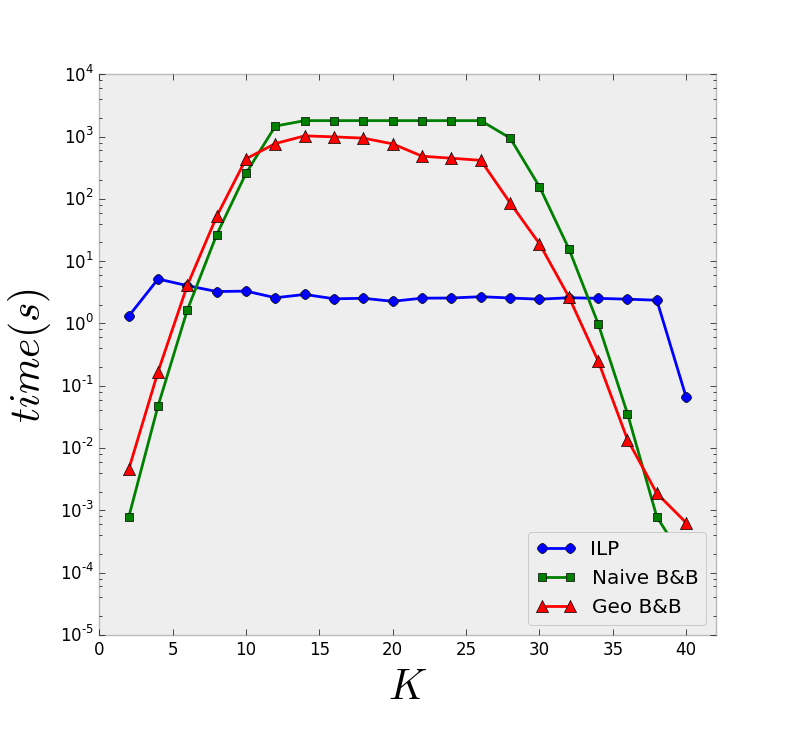
\includegraphics[width=0.9\linewidth]{Pictures/n40} 
    \caption{$N=40$} 
    \label{fig:fixed_n:d} 
  \end{subfigure} 
  \vspace{2ex}
  \begin{center}
  \textcolor{blue}{\cmark}\ -- Integer Linear Programming \quad   \textcolor{red}{\tmark}\ -- Delaunay Assisted B\&B\quad \textcolor{OliveGreen}{\smark}\ -- Naive B\&B
  \end{center}
  \caption{CPU-time for different values of $N$ with varying $K$}
  \label{fig:fixed_n} 
\end{figure}


\noindent
The Integer Linear Programming approach seems to be the fastest approach for most cases, and seems independent to the value of $K$. The exceptions to this seem to be smaller values of $N$, as well as the smallest and largest values of $K$. This happens because the implicit enumeration methods only need to enumerate a very small number of combinations.
As for the branch-and-bound algorithms, the Delaunay-assisted approach is slower than the Naïve implementation in these test cases. However it should be noted that for each $N$, the Delaunay-assisted algorithm peaks before the expected value of $K=N/2$. This is justified due to the fact that the Delaunay triangulation has an overhead which can take advantage for in larger values of $K$.
Furthermore, the fact that the Naïve implementation had no test for the middle values of $K$ for $N=40$ that ended before the time-out mark is noteworthy.
It is also worth noting that The Delaunay-assisted approach showed a lot more variance between tests, often taking much lower values than the mean. However, for the tests performed, two runs had values much larger than the Naïve approach, approximating the Delaunay-assisted algorithm's mean to the Naïve approach.

The time required for each test limited the number of tests performed. Because of this, the results may not be statistically meaningful. 
This could mean that the Delaunay-assisted approach is only preferable for values of $N$ and $K$ to which neither approach is usable in real-time. Due to the small number of tests for large values of $N$, this result may not be statistically meaningful, but it is noteworthy.

\section{Discussion}
The algorithms in this chapter have some drawbacks when used in a web application. Not only were the running times too large to be used in real-time, taking minutes and even hours for small instances with 40 points at most, but they also required some a priori knowledge about the number of clusters on a given window. This is infeasible, since there is no efficient way to infer how many clusters there are in a new region, without testing for all possible values of $K$. The algorithm should be able to calculate the final number of selected points, constrained to a minimum distance factor between them. This can be achieved by solving \emph{Geometric Disk Cover} problem described in Section \ref{ilp2}. The next chapter describes in detail a way to solve this problem in regards to the final application.

\chapter{Future Work}
\label{chap:future}
\lhead{Chapter \ref{chap:future}. \emph{\nameref{chap:future}}}
\section{Integration in a Visualisation Framework}
\paragraph{}
The final objective of this study is to integrate an algorithm in a web application that can display the most representative set. There is, however, a time constraint to do this. The feedback time on the application needs to be as small as possible while still delivering an acceptable set of points, in order to not lose engagement from the user.
\paragraph{}
The application will display a rectangular window, showing a cut of geographical region containing a set of points. The algorithm chosen will need to be able to choose a representative set of points within the cut quickly, as well as be able to recalculate a new set points for a new cut, resulting from panning or zooming the display window over the region.
\paragraph{}
The algorithm serve as the middleware responsible for filtering the response of a GIS server to a Web Map Service, or WMS request. WMS lists the geographic coordinates of the points to be represented in an image by the coordinates mapped into orthogonally organised pixels on an image displaying the cut of the region requested by the application.
The candidate algorithms will be tested and benchmarked using data from the Open Street Map project. The project features large quantities of open source geographic data, as well as a versatile API for fetching data in the WMS standard.
\section{Heuristic Approaches}
\paragraph{}
Optimal solution algorithms, and their slow time performance, makes them a poor choice for real-time applications. As such, heuristic algorithms that provide good but not optimal solution in faster time are more likely the most appropriate approach.
Since a lot of complex structures have already been explored and implemented in the implicit enumeration approaches, a lot of the concepts and methods can be repurposed and reused when experimenting and researching heuristic approaches. 
\change{
	\paragraph{}
	For instance, since the two interactions with any calculated solution will be panning and zooming, some new solutions may share some points. If that is the case, calculating a solution after a small pan or zoom may reuse the previously calculated region as a starting point, only adding the new points, and removing the previously calculated ones.
	\paragraph{}
	An extension to this method may include calculating a larger area than the queried one, so that a small pan and/or zoom include already calculating data. After the window moves, the new adjacent regions can be calculated. This way, the user should never see the window without processed data, and the program will only calculate areas outside the vision range of the window.
}
	\section {Approximation Algorithms}
\change{
	\paragraph{}
	Approximation algorithms are used to used in optimisation as a means to achieve a valid solution within a guaranteed minimum factor of quality to the optimal solution. Ideally, the approximation is optimal up to a constant factor, the smaller the better. Approximation algorithms have been found and described by \citet{approx}, that give an approximation with a factor of $3.16$ to the optimal solution of \emph{p-center} problem.
}
%
%\section{Uniformity}
%\paragraph{}
%Another measure of quality for a solution is its \emph{uniformity}. Uniformity is defined mathematically in a set of points as the distance between the closest pair of points. The most representative subset $U$ of a larger set $N$ relative to its uniformity will be the subset of $N$ that has the highest value for the distance of its closest pair. Like coverage, the concept of uniformity is frequent in the field of optimisation. Maximising uniformity can be formally defined as:
%
%\begin{equation}
%\max_{U \in N}{\min_{\substack{u_i,u_j \in U \\ u_i \neq u_j}}{\lVert u_i-u_j \rVert}}
%\end{equation}
%
%\noindent
%Where $N$ is the initial set of points in $\mathbb{R}^2$, $U$ is the most uniform subset in $N$, and $\lVert \cdot \rVert$ is the Euclidean distance between two points. The maximum uniformity is the most representative set.
\cleardoublepage
\chapter{Conclusion}
\label{chap:conc}
\lhead{Chapter \ref{chap:conc}. \emph{\nameref{chap:conc}}}
\vspace{-15pt}
In this thesis, we designed algorithms to select representative subsets from large quantities of geographic points. The algorithm must be able to handle panning and zooming motions along the geographic region displayed, as well as be efficient enough to be integrated in the back-end of a real-time Web application. 

We started by defining representation as finding the optimal solution to the \emph{$k$-centre} problem. To solve this problem, two different incremental branch-and-bound approaches were implemented. We then compared the performance of these approaches and one formulation of the problem in integer linear programming to ascertain if the problem could be solved in real-time. The results showed not only that optimal approaches are not efficient to meet the time requirements of the application, but also that the problem required a priori information about the number of point clusters in the region.

In a second phase, we redefine the representation problem as to find the solution to the \emph{geometric disk cover} problem instead. This new approach manages to compute the cardinality of the final subset with no information about the region. To solve this problem, we implemented two versions of an approximation algorithm, both of which calculated subsets very efficiently, with a guarantee of approximation to the optimal value. We then performed some tests to determine the most efficient solution. Additionally, we used heuristic approaches to further speed up the algorithm and reduce its memory usage, but without guarantee of approximation.

Throughout this thesis, we found that interpreting the representation problem as \emph{geometric disk cover} problem, and solve it with an approximation algorithm is an efficient way to be applied in the context of a real-time web application. We also found viable solutions for solving larger instances of the problem.

\section{Future Work}
The next step for the web application developer is to integrate the algorithms described and implemented during this thesis. Since the algorithms are already implemented taking into account their place in the architecture of the final product, the inputs and outputs are already conformed to the specifications given. Full integration requires that the communication layer, as well as the proper protocol request and response parsers are implemented.

Although the results were satisfactory, it may still be possible to develop more efficient algorithms. The bottleneck for our final approaches lies in the proximity graph building stage, particularly performing the various range search queries to establish neighbouring points. This means that implementing more efficient range search structures is a good strategy to find better solutions. Furthermore, since the evaluation of the results may depend of the perspective of the user, new solutions might require different interpretations on the concept of representation, such as the notion of uniformity or other similar metrics. 

\end{document}